Stopping criteria are the essential part of the automatic Bayesian cubature algorithm which computes the integral of a black-box function for the user given error tolerance just using the function sample values at predetermined sample locations.



\paragraph{Normality test using QQ-plot:}
The Bayesian cubature algorithms assume that the integrand arises from a Gaussian process. This means that the integrand values, $\vf$, satisfy a multivariate Gaussian distribution, as in \eqref{eqn:fGaussDist}.  The transformed data, $\vZ = \frac 1n \mV \mLambda^{-\frac 12} \mV^H(\vf - m \vone)$, has zero mean and is also uncorrelated because
\begin{align*}
\Ex\left[\vZ \right] &= 
\frac 1n \mV \mLambda^{-\frac 12} \mV^H(\Ex\left[\vf\right] - m \vone) 
\\
& = 0
\end{align*}
\begin{align*}
\cov (\vZ) 
&= \frac {1}{n^2} \Ex\left[  
\mV \mLambda^{-\frac 12} \mV^H (\vf - m \vone)
(\vf - m \vone)^T \mV \mLambda^{-\frac 12} \mV^H
\right]
\\
&=
\frac {1}{n^2} \mV \mLambda^{-\frac 12} \mV^H 
\Ex \biggl[ (\vf - m \vone)
(\vf - m \vone)^T \biggr] \mV \mLambda^{-\frac 12} \mV^H
\\ % Note : \mV^h \mV = n
&=
\frac{1}{n^2} \mV \mLambda^{-\frac 12} \mV^H 
\frac 1n \mV \mLambda \mV^H \mV \mLambda^{-\frac 12} \mV^H
\\
&=
\frac{1}{n^3} \mV \mLambda^{-\frac 12} (n) \mLambda (n) \mLambda^{-\frac 12} \mV^H
= \mathsf{I}
\end{align*}
Thus, the elements of $\vZ$ are IID standard Gaussian random variables.  
In practice, using the estimated $m_\MLE$ further simplifies, 
\begin{align}
\nonumber
\vZ &= \frac 1n \mV \mLambda^{-\frac 12} \mV^H(\vf - m \vone) \\
\nonumber
 &= \frac 1n \mV \mLambda^{-\frac 12} (\mV^H \vf - \frac{\tilde{f}_1}{n} \mV^H \vone) 
\\
\label{eqn:normalize}
 &= \frac 1n \mV \mLambda^{-\frac 12} \left(\mV^H \vf - \tilde{f}_1 \begin{pmatrix}1, 0, \hdots, 0 \end{pmatrix}^T \right) 
\end{align}

For the given function values of the integrand and the samples locations, first we obtain the parameters. The obtained parameters: shape parameter $\theta$,  scale parameter $s$ and the kernel order $r$ are used to formulate the matrix $\mV$. Then the eigen matrix $\mV$ is used to normalize the function values as shown in \eqref{eqn:normalize}.
We use the following three integrands to validate our hypothesis.  

\paragraph{
Example-1 Exponential of Cosine:}
\begin{equation*}
\int_{[0,1]^{d}}  \exp( - \sum_{i=1}^d\cos(\norm{\vt}) ) \, \dif \vt
= \ \int_{[0,1]^{d}} 
f(\vx) \, 
\dif \vx 
\end{equation*}
This is a smooth and periodic function and is periodic in the interval $[0,1]$. The Figure \ref{fig:expcos_plots} shows the objective function on the left and the QQ-plot of the transformed $\vZ$ coefficients. In the supplement notebook \code{gaussian\_diagnostics\_demo.ipynb} additional plots with different $n$ values can be found. As observed in the QQ-plot, $\vZ$ shows some straits of normality but not perfect. We observe that the normality seems higher for the lower $n$ values. Plot of the objective function looks smooth with no local minimums. Also the integrand is very smooth and possibly the integrand does not belong to the middle of the the sample space spanned by the basis functions.
\begin{figure}[ht]
	\centering
	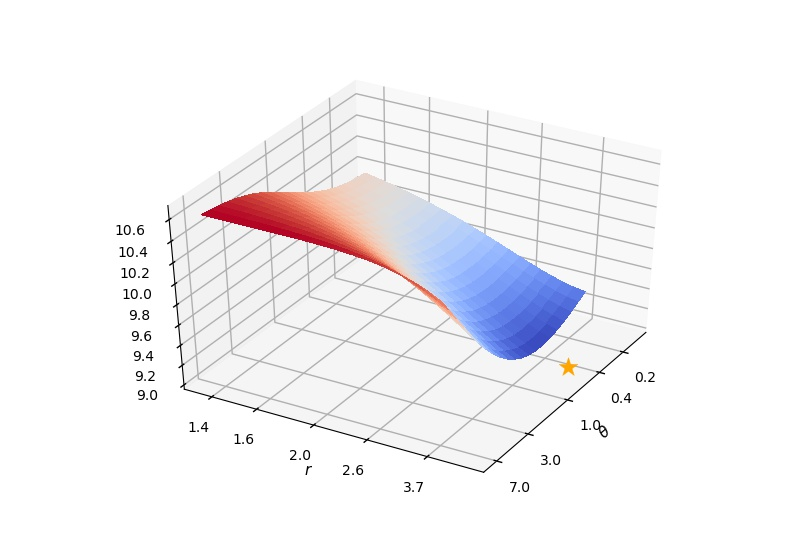
\includegraphics[width=0.45\linewidth]{BayesCub/figures/ExpCos-ObjFun_n-64_d-3_case-0.jpg} \quad 
	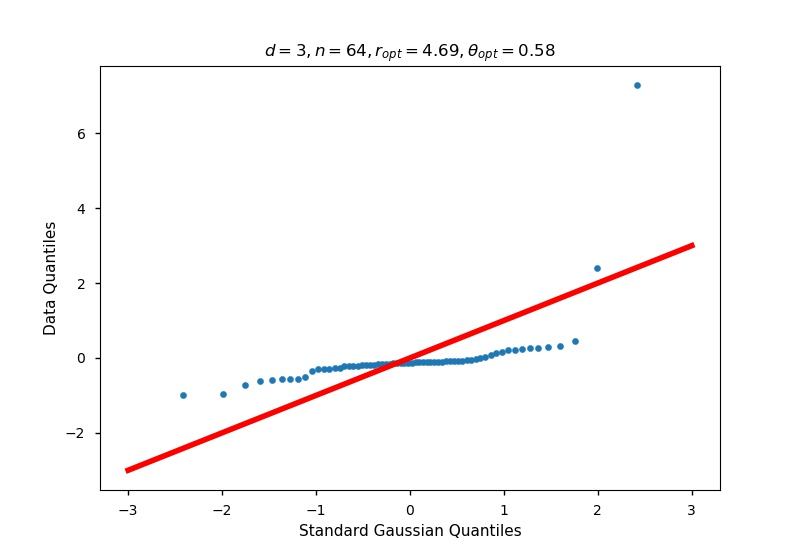
\includegraphics[width=0.45\linewidth]{BayesCub/figures/ExpCos-QQPlot_n-64_d-3_case-0.jpg}
	\caption{Exp(cos) function $d=3, n=64, case=0$: Objective function (left);  QQ plot (right).  These plots can be conditionally reproduced using \code{gaussian\_diagnostics\_demo.ipynb}}
	\label{fig:expcos_plots}
\end{figure}




\paragraph{
Example-2 Custom random function:}

Unlike the previous integrand, we construct an integrand in particular using the basis functions that span our sample space. This ensure the integrand belongs to the middle of the sample space. To simplify with the practical implementation we truncate the shift invariant kernel's infinite series to a finite series. But the coefficient in the finite sum are randomly chosen. Randomly choosing the coefficients avoid any accidental bias in the constructed integrand. This helps to simplify the basis function count to a finite value. 
\[
\begin{aligned}
f(\vx) & = \widehat{f}_0  \\
& + \sum_{\vk \in \{1, \ldots, N\}^d} \Bigl[\widehat{f}_c(\vk) \cos(2\pi \vk^T \vx) + \widehat{f}_s(\vk)\sin(2\pi \vk^T \vx)\Bigr] \\
& \qquad  \widehat{f}_0, \  \widehat{f}_c(\vk), \ \widehat{f}_s(\vk) \IIDsim \cn\biggl(0,a^{\norm[0]{\vk}} b^{d-\norm[0]{\vk}}\prod_{k_j \ne 0} k_j^{-r}\biggr) \\
& \qquad \theta = a/b,  \qquad N = 256
\end{aligned}
\]%

Unlike the previous integrand, this ones shows much better QQ-plot with the higher normality. This observation strengthens our hypothesis, if the integrand arises from the middle of the sample space then the accuracy of the algorithm also much higher.
\begin{figure}[ht]
	\centering
	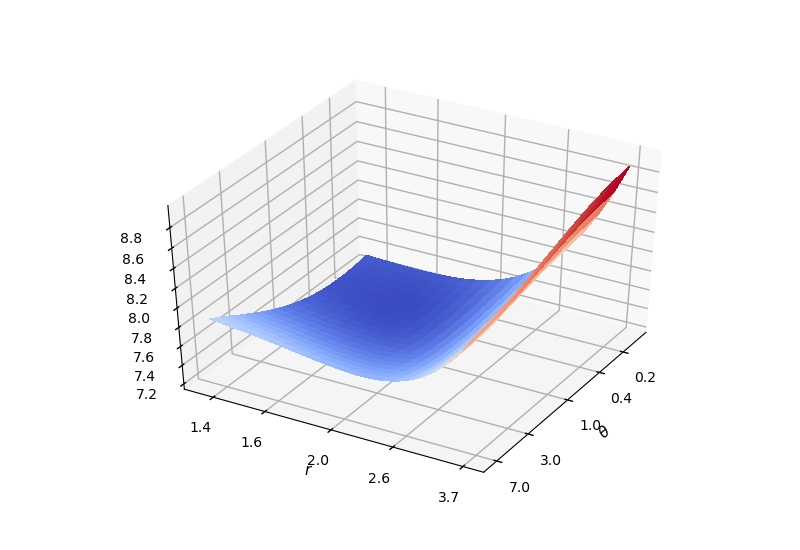
\includegraphics[width=0.45\linewidth]{BayesCub/figures/rand-ObjFun_n-64_d-2_r-150.0_th-25.0_case-0.jpg} \quad 
	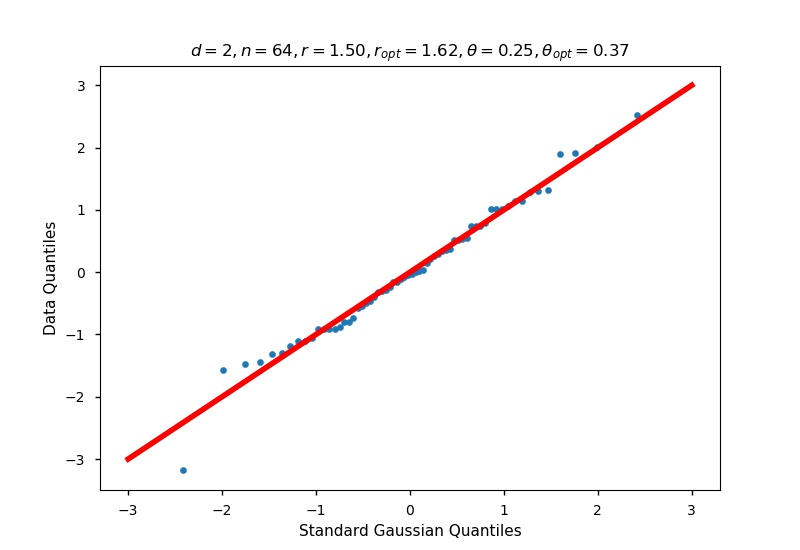
\includegraphics[width=0.45\linewidth]{BayesCub/figures/rand-QQPlot_n-64_d-2_r-150.0_th-25.0_case-0.jpg}
	\caption{Random function $d=2, n=64, case=0$: Objective function (left);  QQ plot (right).  These plots can be conditionally reproduced using \code{gaussian\_diagnostics\_demo.ipynb}}
	\label{fig:rand_plots}
\end{figure}

\paragraph{
Example-3 Keister integrand:}
\begin{equation*}
\int_{\reals^d} \cos(\norm{\vt})\exp(-\norm{\vt}^2) \, \dif \vt
= \ \int_{[0,1]^{d}} 
f(\vx) \, 
\dif \vx 
\end{equation*}
In contrast to the previous two integrands, Keister integrand is also smoother but not periodic. It also has higher number of derivatives. Keister integrand 
\begin{figure}[ht]
	\centering
	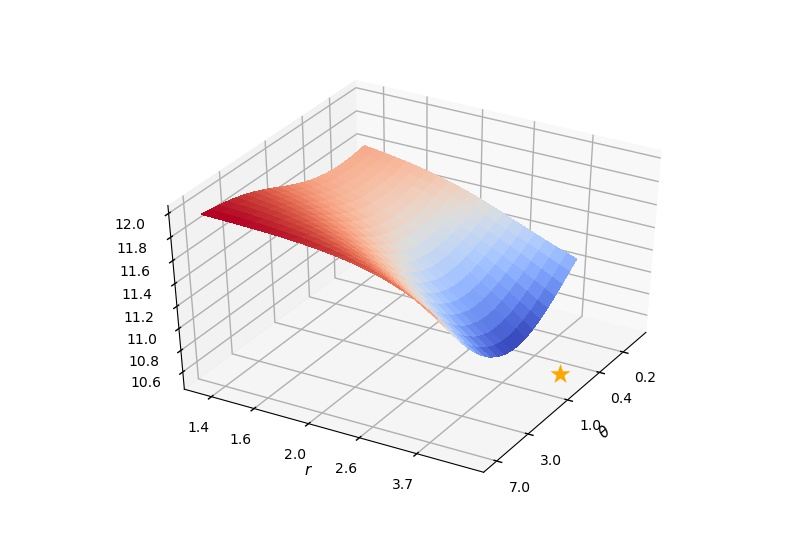
\includegraphics[width=0.45\linewidth]{BayesCub/figures/Keister-ObjFun_n-64_d-3_case-0.jpg} \quad 
	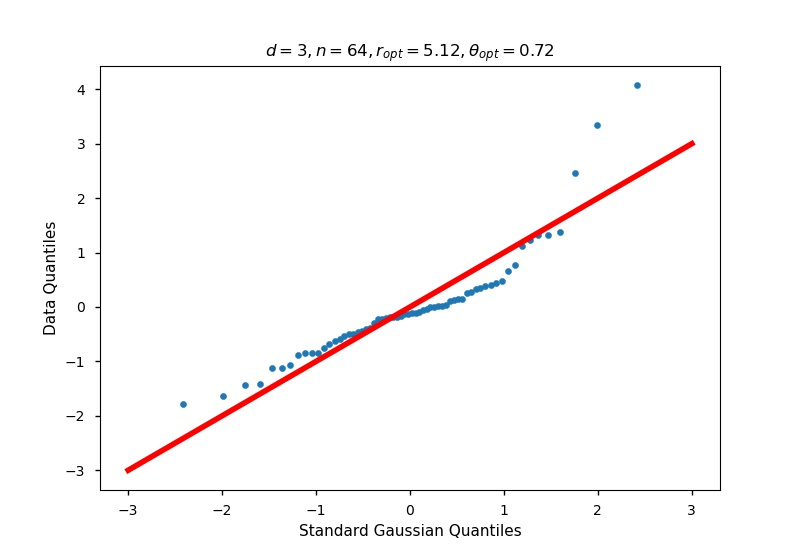
\includegraphics[width=0.45\linewidth]{BayesCub/figures/Keister-QQPlot_n-64_d-3_case-0.jpg}
	\caption{Keister integrand $d=3, n=1024, case=0$: Objective function (left);  QQ plot (right).  These plots can be conditionally reproduced using \code{gaussian\_diagnostics\_demo.ipynb}}
	\label{fig:keister_plots}
\end{figure}